\section{Discussions}\label{chapter-ML-section-discussion}
Les effets
de l'empilement,
de la reconstruction des particules,
des faux taus hadroniques,
de la séparation des canaux et
de l'intervalle de masse
sur les prédictions de masse
sont discutées ci-après.
Lors de cette thèse, ces effets ont été étudiés en parallèle de l'exploration des hyper-paramètres présentée en section~\ref{chapter-ML-section-hyperparameters} avec des modèles divers.
À des fins de cohérence dans la comparaison des effets,
nous utilisons ici le modèle B sélectionné précédemment comme référence.
\subsection{Effet de l'empilement}
\def\Bnpu{$\text{B}^\text{0PU}$}
Dans les travaux de \citeauthor{BARTSCHI201929}~\cite{BARTSCHI201929},
l'empilement (PU, \emph{Pile-Up}) n'est pas considéré.
Nous avons donc souhaité déterminer l'effet de l'empilement sur les prédictions de notre modèle.
Pour cela, les mêmes événements que ceux décrits en section~\ref{chapter-ML-section-evt_gen} ont été générés sans empilement.
Un DNN, noté \Bnpu, est entraîné sur ces événements sans empilement.
Les hyper-paramètres de \Bnpu\ sont ceux de B, à l'exception des variables d'entrée auxquelles \Npu\ est retiré, car $\Npu=0$ pour tous les événements sans empilement.
La réponse de \Bnpu\ sur les événements de test sans empilement est représentée sur la figure~\ref{subfig-reponse_model_PU_00}.
La réponse moyenne du modèle est de $\num{1.00}\pm\num{0.05}$ pour $m_{\higgsML}$ entre \SI{70}{\GeV} et \SI{600}{\GeV} avec une résolution relative de l'ordre de \SI{22}{\%} à basse masse et \SI{10}{\%} à haute masse.
\begin{figure}[h]
\centering

\subcaptionbox{Réponse de \Bnpu\ sur les événements sans empilement.\label{subfig-reponse_model_PU_00}}[.45\textwidth]
{\includegraphics[width=.45\textwidth]{\PhDthesisdir/plots_and_images/my_plots/ML/from_ML_plots/DNNs_for_discussion/PU/trained_wo_PU_wo_Npu/test_wo_PU/model_response-NN-activation-softplus-batch_size-2048-mape-Adam-gu-inclusive-3-layers-1000-neurons.pdf}\vspace{-.5\baselineskip}}
\hfill
\subcaptionbox{Réponse de \Bnpu\ sur les événements avec empilement.\label{subfig-reponse_model_PU_01}}[.45\textwidth]
{\includegraphics[width=.45\textwidth]{\PhDthesisdir/plots_and_images/my_plots/ML/from_ML_plots/DNNs_for_discussion/PU/trained_wo_PU_wo_Npu/test_on_PU/model_response-NN-activation-softplus-batch_size-2048-mape-Adam-gu-inclusive-3-layers-1000-neurons.pdf}\vspace{-.5\baselineskip}}

\caption{Réponses du modèle \Bnpu\ sur les événements sans et avec empilement.}
\label{fig-reponse_model_0PU}
\end{figure}
\par
Cependant, la réponse de \Bnpu\ est dégradée sur des événements contenant de l'empilement, figure~\ref{subfig-reponse_model_PU_01}.
La réponse médiane se situe en effet à \num{1.13} à $m_{\higgsML}=\SI{100}{\GeV}$ et diminue à \num{0.83} à $m_{\higgsML}=\SI{800}{\GeV}$ avec empilement contre \num{1.00} et \num{0.83} sans empilement.
La résolution relative à basse masse est de l'ordre de \SI{25}{\%} avec empilement.
\par
L'empilement peut être considéré comme un bruit blanc, dont l'énergie moyenne est reliée à \Npu.
L'énergie portée par $L_1$ et $L_2$, les éléments visibles de la désintégration de \higgsML,
est en revanche reliée à $m_{\higgsML}$.
À haute masse, l'énergie de $L_1$ et $L_2$ est grande par rapport à celle de l'empilement.
Les prédictions de \Bnpu\ ne sont alors pas perturbées,
menant à des performances similaires à celles du cas sans empilement.
Lorsque $m_{\higgsML}$ diminue,
l'énergie disponible pour $L_1$ et $L_2$ est moindre
et
le bruit d'empilement est alors compétitif.
Le modèle \Bnpu\ n'est pas entraîné pour traiter ce bruit et ses prédictions sont perturbées.
Il est donc primordial d'inclure l'empilement dans l'entraînement dans l'optique d'une utilisation de nos modèles dans les analyses de CMS.
\par
La réponse du modèle B, entraîné avec empilement, peut être comparée
dans le cas d'événements sans empilement, figure~\ref{subfig-reponse_model_PU_10},
au cas d'événements avec empilement, figure~\ref{subfig-reponse_model_PU_11} (identique à~\ref{subfig-reponse_model_B}).
Le profil d'empilement utilisé pour générer les événements d'entraînement est celui de l'année 2017.
Or, il apparaît que le modèle B est peu sensible au retrait de l'empilement, les réponses étant similaires sur les figure~\ref{subfig-reponse_model_PU_10} et~\ref{subfig-reponse_model_PU_11}.
L'utilisation de B sur des événements dont le profil d'empilement est légèrement différent de celui de l'année 2017,
comme c'est le cas pour les autres années du Run~II (2016, 2018)
est ainsi directement envisageable.
\begin{figure}[h]
\centering

\subcaptionbox{Réponse de B sur les événements sans empilement.\label{subfig-reponse_model_PU_10}}[.45\textwidth]
{\includegraphics[width=.45\textwidth]{\PhDthesisdir/plots_and_images/my_plots/ML/from_ML_plots/DNNs_for_discussion/PU/trained_on_PU/test_wo_PU/model_response-NN-ADAM_glorot_uniform-activation-softplus-batch_size-2048-mape-Adadelta-u-inclusive-3-layers-1000-neurons.pdf}\vspace{-.5\baselineskip}}
\hfill
\subcaptionbox{Réponse de B sur les événements avec empilement.\label{subfig-reponse_model_PU_11}}[.45\textwidth]
{\includegraphics[width=.45\textwidth]{\PhDthesisdir/plots_and_images/my_plots/ML/from_ML_plots/trained_NNs_FastSim/DeepTau-inclusive/PuppiMET_with_METcov_j1j2jr_Nnu_Npu/model_response-NN-ADAM_glorot_uniform-activation-softplus-batch_size-2048-mape-Adadelta-u-inclusive-3-layers-1000-neurons.pdf}\vspace{-.5\baselineskip}}

\caption{Réponses du modèle B sur les événements sans et avec empilement.}
\label{fig-reponse_model_1PU}
\end{figure}
\subsection{Effet de la reconstruction des particules}
\def\Bgenleg{$\text{B}^\text{gen}$}
La reconstruction des particules est présentée dans le chapitre~\refChLHCCMS.
Son effet peut être caractérisé par l'étude du modèle \Bgenleg,
ayant les mêmes hyper-paramètres que B mais entraîné en utilisant les objets générés au lieu de ceux reconstruits pour $L_1$, $L_2$ et \MET, \ie\ pour les trois objets physiques liés à la désintégration des leptons~\tau\ (deux parties visibles $L_1$ et $L_2$ et \MET\ pour les neutrinos).
En particulier, les valeurs de $\vpT^{L_1}$, $\vpT^{L_2}$ et \vMET\ correspondent exactement à la réalité.
Il s'agit donc du cas où les objets physiques issus de \higgsML\ sont parfaitement reconstruits.
Toutes les autres variables, y compris la matrice de covariance de \MET, restent celles obtenues avec les objets reconstruits.
\par
La figure~\ref{fig-reponse_model_1GENleg} montre les réponses du modèle \Bgenleg\ sur les événements avec reconstruction parfaite et réelle.
Dans le cas d'une reconstruction parfaite,
la réponse médiane de \Bgenleg\ est de l'ordre de $\num{1.01}\pm\num{0.02}$ de \num{70} à \SI{800}{\GeV}.
La résolution relative est quant à elle de l'ordre de \SI{3}{\%} soit près de sept fois mieux que B.
\begin{figure}[h]
\centering

\subcaptionbox{Réponse de \Bgenleg\ dans le cas d'une reconstruction parfaite.\label{subfig-reponse_model_GENleg_10}}[.45\textwidth]
{\includegraphics[width=.45\textwidth]{\PhDthesisdir/plots_and_images/my_plots/ML/from_ML_plots/DNNs_for_discussion/Reco_effect/GENleg_with_METcov_j1j2jr_Nnu_Npu/model_response-NN-activation-softplus-batch_size-2048-mape-Adam-gu-inclusive-3-layers-1000-neurons.pdf}\vspace{-.5\baselineskip}}
\hfill
\subcaptionbox{Réponse de \Bgenleg\ dans le cas d'une reconstruction réelle.\label{subfig-reponse_model_GENleg_11}}[.45\textwidth]
{\includegraphics[width=.45\textwidth]{\PhDthesisdir/plots_and_images/my_plots/ML/from_ML_plots/DNNs_for_discussion/Reco_effect/GENleg_with_METcov_j1j2jr_Nnu_Npu/test_on_reco/model_response-NN-activation-softplus-batch_size-2048-mape-Adam-gu-inclusive-3-layers-1000-neurons.pdf}\vspace{-.5\baselineskip}}

\caption[Réponses du modèle \Bgenleg\ avec reconstruction parfaite ou réelle.]{Réponses du modèle \Bgenleg\ dans le cas d'une reconstruction des particules parfaite et réelle.}
\label{fig-reponse_model_1GENleg}
\end{figure}
\par
Les DNNs sont donc en mesure
de comprendre la physique des événements $\higgsML\to\tau\tau$
afin d'estimer $m_{\higgsML}$
à partir des objets physiques générés
correspondant aux objets effectivement reconstruits par le détecteur.
Cependant, comme le montre la figure~\ref{subfig-reponse_model_GENleg_11},
l'utilisation de \Bgenleg\ sur les variables reconstruites, effectivement accessibles expérimentalement, ne permet pas d'obtenir $m_{\higgsML}$.
En effet, la réponse moyenne de \Bgenleg\ avec ces variables est inférieure à \num{1} et de l'ordre de \num{0.7} à haute masse.
De plus, la résolution relative est de l'ordre de \SI{40}{\%}.
Une des tâches des DNNs est donc de corriger cet effet de reconstruction.
\subsection{Effet des faux taus hadroniques}
La phénoménologie des événements contenant une paire de leptons~\tau\ est décrite dans le chapitre~\refChMSSM.
Ces leptons peuvent se désintégrer hadroniquement en tau hadronique (\tauh) ou leptoniquement en électron (\ele) ou en muon (\mu).
%Ces désintégrations s'accompagnent de l'émission de un (cas hadronique) ou deux (cas leptoniques) neutrinos.
Il existe ainsi six canaux différents dans les événements avec une paire de leptons~\tau, pouvant être répartis en trois groupes:
\begin{itemize}
\item complètement hadronique: \tauh\tauh, avec deux \tauh;
\item semi-leptoniques: \mu\tauh\ et \ele\tauh, ou simplement $\ell\tauh$, avec un \tauh;
\item leptoniques: \mu\mu, \ele\mu\ et \ele\ele, ou simplement $\ell\ell$, sans \tauh.
\end{itemize}
\par
Les faux taus hadroniques (\ftauhs) sont des objets physiques tels que des électrons, des muons et surtout des jets identifiés à tort comme des \tauh.
Ils représentent près de \SI{70}{\%} des événements dans le canal \tauh\tauh, \SI{38}{\%} dans le canal \mu\tauh\ et \SI{68}{\%} dans le canal \ele\tauh.
Les \ftauhs\ sont particulièrement difficiles à modéliser dans les simulations~\cite{CMS-NOTE-2018-257,CMS-NOTE-2019-170}.
\par
L'identification des \tauh\ est réalisée dans nos travaux à l'aide de l'algorithme \DEEPTAU~\cite{CMS-DP-2019-033},
qui présente un faible taux de mauvaise identification des \tauh, inférieur à \SI{1}{\%}.
Cependant, une autre méthode d'identification des \tauh, basée sur un arbre de décision (BDT), peut être utilisée et présente un taux de mauvaise identification de jets en tant que \tauh\ pouvant atteindre \SI{4}{\%}~\cite{Khachatryan:2015dfa}.
Une sélection plus riche en \ftauhs\ est ainsi obtenue.
\par
Les réponses du modèle B sur chacun des trois groupes de canaux (hadronique, semi-leptoniques et leptoniques) sont représentées figure~\ref{fig-fakes_B_tt-lt-ll} pour les deux ensembles de sélection des \tauh.
\begin{figure}[p]
\centering

\def\localch{tt}
\subcaptionbox{Canal \GetChannelStr{\localch}, \DEEPTAU.\label{subfig-B_few_fakes_\localch}}[.45\textwidth]
{\includegraphics[width=.45\textwidth]{\PhDthesisdir/plots_and_images/my_plots/ML/from_ML_plots/DNNs_for_discussion/Channel_split/train_on_inclusive/test_on_\localch/model_response-NN-ADAM_glorot_uniform-activation-softplus-batch_size-2048-mape-Adadelta-u-inclusive-3-layers-1000-neurons.pdf}\vspace{-.5\baselineskip}}
\hfill
\subcaptionbox{Canal \GetChannelStr{\localch}, BDT.\label{subfig-B_more_fakes_\localch}}[.45\textwidth]
{\includegraphics[width=.45\textwidth]{\PhDthesisdir/plots_and_images/my_plots/ML/from_ML_plots/DNNs_for_discussion/Fakes_no_DeepTau/trained_on_not_fakes/inclusive_train_test_on_\localch/model_response-NN-ADAM_glorot_uniform-activation-softplus-batch_size-2048-mape-Adadelta-u-inclusive-3-layers-1000-neurons.pdf}\vspace{-.5\baselineskip}}

\def\localch{lt}
\subcaptionbox{Canaux \GetChannelStr{\localch}, \DEEPTAU.\label{subfig-B_few_fakes_\localch}}[.45\textwidth]
{\includegraphics[width=.45\textwidth]{\PhDthesisdir/plots_and_images/my_plots/ML/from_ML_plots/DNNs_for_discussion/Channel_split/train_on_inclusive/test_on_\localch/model_response-NN-ADAM_glorot_uniform-activation-softplus-batch_size-2048-mape-Adadelta-u-inclusive-3-layers-1000-neurons.pdf}\vspace{-.5\baselineskip}}
\hfill
\subcaptionbox{Canaux \GetChannelStr{\localch}, BDT.\label{subfig-B_more_fakes_\localch}}[.45\textwidth]
{\includegraphics[width=.45\textwidth]{\PhDthesisdir/plots_and_images/my_plots/ML/from_ML_plots/DNNs_for_discussion/Fakes_no_DeepTau/trained_on_not_fakes/inclusive_train_test_on_\localch/model_response-NN-ADAM_glorot_uniform-activation-softplus-batch_size-2048-mape-Adadelta-u-inclusive-3-layers-1000-neurons.pdf}\vspace{-.5\baselineskip}}

\def\localch{ll}
\subcaptionbox{Canaux \GetChannelStr{\localch}, \DEEPTAU.\label{subfig-B_few_fakes_\localch}}[.45\textwidth]
{\includegraphics[width=.45\textwidth]{\PhDthesisdir/plots_and_images/my_plots/ML/from_ML_plots/DNNs_for_discussion/Channel_split/train_on_inclusive/test_on_\localch/model_response-NN-ADAM_glorot_uniform-activation-softplus-batch_size-2048-mape-Adadelta-u-inclusive-3-layers-1000-neurons.pdf}\vspace{-.5\baselineskip}}
\hfill
\subcaptionbox{Canaux \GetChannelStr{\localch}, BDT.\label{subfig-B_more_fakes_\localch}}[.45\textwidth]
{\includegraphics[width=.45\textwidth]{\PhDthesisdir/plots_and_images/my_plots/ML/from_ML_plots/DNNs_for_discussion/Fakes_no_DeepTau/trained_on_not_fakes/inclusive_train_test_on_\localch/model_response-NN-ADAM_glorot_uniform-activation-softplus-batch_size-2048-mape-Adadelta-u-inclusive-3-layers-1000-neurons.pdf}\vspace{-.5\baselineskip}}

\caption[Effet des \ftauhs\ sur la réponse du modèle B.]{Réponses du modèle B sur les différents types de canaux avec une quantité variable de \ftauhs.}
\label{fig-fakes_B_tt-lt-ll}
\end{figure}
Quel que soit le groupe d'état final, les réponses pour $m_{\higgsML}>\SI{600}{\GeV}$ ne sont pas affectées par la sélection des \tauh.
En effet, pour de hautes valeurs de $m_{\higgsML}$, les \tauh\ ont des impulsions suffisamment élevées pour être correctement sélectionnés par la séquence d'analyse.
À basse masse en revanche,
les impulsions des \ftauhs\ sont compétitives vis-à-vis de celles des vrais \tauh.
La séquence d'analyse forme alors des dileptons contenant des \ftauhs.
La réponse du modèle s'en retrouve modifiée,
jusqu'à \SI{20}{\%} de plus
pour des masses entre \SI{100}{\GeV} et \SI{600}{\GeV}.
L'effet le plus important se situe à très basse masse où la résolution est fortement dégradée.
\begin{figure}[p]
\centering

\def\localch{tt}
\subcaptionbox{Canal \GetChannelStr{\localch}, \DEEPTAU.\label{subfig-diffs_B_few_fakes_\localch}}[.45\textwidth]
{\includegraphics[width=.45\textwidth]{\PhDthesisdir/plots_and_images/my_plots/ML/from_ML_plots/DNNs_for_discussion/Channel_split/train_on_inclusive/test_on_\localch/model_response_diff_lowmass-NN-ADAM_glorot_uniform-activation-softplus-batch_size-2048-mape-Adadelta-u-inclusive-3-layers-1000-neurons.pdf}\vspace{-.5\baselineskip}}
\hfill
\subcaptionbox{Canal \GetChannelStr{\localch}, BDT.\label{subfig-diffs_B_more_fakes_\localch}}[.45\textwidth]
{\includegraphics[width=.45\textwidth]{\PhDthesisdir/plots_and_images/my_plots/ML/from_ML_plots/DNNs_for_discussion/Fakes_no_DeepTau/trained_on_not_fakes/inclusive_train_test_on_\localch/model_response_diff_lowmass-NN-ADAM_glorot_uniform-activation-softplus-batch_size-2048-mape-Adadelta-u-inclusive-3-layers-1000-neurons.pdf}\vspace{-.5\baselineskip}}

\def\localch{lt}
\subcaptionbox{Canaux \GetChannelStr{\localch}, \DEEPTAU.\label{subfig-diffs_B_few_fakes_\localch}}[.45\textwidth]
{\includegraphics[width=.45\textwidth]{\PhDthesisdir/plots_and_images/my_plots/ML/from_ML_plots/DNNs_for_discussion/Channel_split/train_on_inclusive/test_on_\localch/model_response_diff_lowmass-NN-ADAM_glorot_uniform-activation-softplus-batch_size-2048-mape-Adadelta-u-inclusive-3-layers-1000-neurons.pdf}\vspace{-.5\baselineskip}}
\hfill
\subcaptionbox{Canaux \GetChannelStr{\localch}, BDT.\label{subfig-diffs_B_more_fakes_\localch}}[.45\textwidth]
{\includegraphics[width=.45\textwidth]{\PhDthesisdir/plots_and_images/my_plots/ML/from_ML_plots/DNNs_for_discussion/Fakes_no_DeepTau/trained_on_not_fakes/inclusive_train_test_on_\localch/model_response_diff_lowmass-NN-ADAM_glorot_uniform-activation-softplus-batch_size-2048-mape-Adadelta-u-inclusive-3-layers-1000-neurons.pdf}\vspace{-.5\baselineskip}}

\def\localch{ll}
\subcaptionbox{Canaux \GetChannelStr{\localch}, \DEEPTAU.\label{subfig-diffs_B_few_fakes_\localch}}[.45\textwidth]
{\includegraphics[width=.45\textwidth]{\PhDthesisdir/plots_and_images/my_plots/ML/from_ML_plots/DNNs_for_discussion/Channel_split/train_on_inclusive/test_on_\localch/model_response_diff_lowmass-NN-ADAM_glorot_uniform-activation-softplus-batch_size-2048-mape-Adadelta-u-inclusive-3-layers-1000-neurons.pdf}\vspace{-.5\baselineskip}}
\hfill
\subcaptionbox{Canaux \GetChannelStr{\localch}, BDT.\label{subfig-diffs_B_more_fakes_\localch}}[.45\textwidth]
{\includegraphics[width=.45\textwidth]{\PhDthesisdir/plots_and_images/my_plots/ML/from_ML_plots/DNNs_for_discussion/Fakes_no_DeepTau/trained_on_not_fakes/inclusive_train_test_on_\localch/model_response_diff_lowmass-NN-ADAM_glorot_uniform-activation-softplus-batch_size-2048-mape-Adadelta-u-inclusive-3-layers-1000-neurons.pdf}\vspace{-.5\baselineskip}}

\caption[Effet des \ftauhs\ sur l'écart des prédictions du modèle B à la valeur vraie.]{Écarts à basse masse du modèle B sur les différents types de canaux avec une quantité variable de \ftauhs.}
\label{fig-diffs_fakes_B_tt-lt-ll}
\end{figure}
\par
La figure~\ref{fig-diffs_fakes_B_tt-lt-ll} montre la différence $\ypred-\ytrue$ entre les prédictions du modèle B et la valeur vraie de $m_{\higgsML}$ pour des valeurs de $m_{\higgsML}$ entre \num{50} et \SI{200}{\GeV} sur chacun des trois groupes de canaux et pour les deux ensembles de sélection des \tauh.
Dans les canaux leptoniques ($\ell\ell$),
figures~\ref{subfig-diffs_B_few_fakes_ll} et~\ref{subfig-diffs_B_more_fakes_ll},
l'effet de la sélection des \tauh\
est moindre que dans les autres canaux.
Il n'y a en effet aucun \tauh\ dans le dilepton, seule la sélection des événements est modifiée.
Un objet physique identifié comme un \tauh\ par le BDT et non par \DEEPTAU\ peut en effet faire basculer l'événement d'un canal à l'autre, si le \tauh\ identifié par le BDT permet de construire un dilepton.
\par
Dans le cas des canaux semi-leptoniques ($\ell\tauh$),
la différence entre \ypred\ de B et \ytrue\ à basse masse est en moyenne inférieure à \SI{10}{\GeV}
pour une sélection des \tauh\ par \DEEPTAU, figure~\ref{subfig-diffs_B_few_fakes_lt}.
La résolution relative est quant à elle inférieure à \SI{25}{\%}.
Lorsque les \tauh\ sont identifiés par le BDT,
figure~\ref{subfig-diffs_B_more_fakes_lt},
le modèle surestime $m_{\higgsML}$ de \SI{25}{\GeV} en moyenne pour $\SI{70}{\GeV} < m_{\higgsML} < \SI{200}{\GeV}$
et de près de \SI{40}{\GeV} à $m_{\higgsML}=\SI{50}{\GeV}$.
La résolution relative est de l'ordre de \SI{25}{\%} au-dessus de \SI{70}{\GeV},
moins bonne qu'avec \DEEPTAU,
et augmente drastiquement pour des masses plus basses, ce qui n'est pas le cas avec \DEEPTAU.
Il s'agit donc de la contribution des \ftauhs.
\par
Dans le canal \tauh\tauh,
figures~\ref{subfig-diffs_B_few_fakes_tt} et~\ref{subfig-diffs_B_more_fakes_tt},
un effet similaire existe.
La résolution relative est toujours de l'ordre de \SI{22}{\%} au-delà de \SI{100}{\GeV},
mais la présence des \ftauhs\ mène à une surestimation moyenne de \SI{30}{\GeV} pour $m_{\higgsML}>\SI{110}{\GeV}$
et pouvant aller jusqu'à \SI{100}{\GeV} pour $m_{\higgsML}\simeq\SI{50}{\GeV}$, soit une erreur de \SI{200}{\%}.
La dégradation de la résolution à très basse masse commence dès \SI{100}{\GeV}, au lieu de \SI{70}{\GeV} pour les canaux $\ell\tauh$.
L'effet des \ftauhs\ est donc plus important que dans les canaux $\ell\tauh$,
ce qui s'explique facilement par la présence de deux \tauh\ au lieu d'un seul.
Pour $m_{\higgsML}=\SI{50}{\GeV}$, la résolution de B sur les événements avec \DEEPTAU\ est également mauvaise.
La sélection des \tauh\ se fait avec $\pT>\SI{40}{\GeV}$, ce qui est difficile à obtenir pour $m_{\higgsML}=\SI{50}{\GeV}$.
Ces événements sont donc peu nombreux et vraisemblablement très contaminés par les \ftauhs.
\par
Les \ftauhs\ introduisent donc un biais important sur une large gamme de masse
et en particulier dans la région des bosons
\Zboson\ ($m_{\Zboson}=\SI{91.2}{\GeV}$)
et
\higgs\ ($m_{\higgs}=\SI{125.1}{\GeV}$).
L'inclusion des \ftauhs\ dans l'entraînement est non triviale, car la masse à prédire n'est pas définie,
les \ftauhs\ n'étant pas des objets physiques provenant de \higgsML.
\subsection{Effet de la séparation des canaux}
\def\Bchsplit#1{\ifthenelse{\equal{#1}{x}}{$\text{B}^{#1}$}{$\text{B}^\text{\GetChannelStr{#1}}$}}
Les modèles construits sont entraînés et testés sur l'ensemble des événements, sans sélection sur le canal.
Or,
il est possible d'entraîner un DNN par canal afin de le spécialiser à la phénoménologie associée
et obtenir, potentiellement, de meilleures estimations de $m_{\higgsML}$.
\par
Les modèles notés \Bchsplit{x} possèdent les mêmes hyper-paramètres que B mais sont entraînés uniquement sur les événements du canal $x$.
\subsubsection{Séparation en six canaux}
Les figures~\ref{fig-tt-mt-et} et~\ref{fig-mm-em-ee} donnent
les réponses des modèles
\Bchsplit{tt},
\Bchsplit{mt},
\Bchsplit{et}
et
\Bchsplit{mm},
\Bchsplit{em},
\Bchsplit{ee}
testés sur leurs canaux respectifs,
comparées à celles de B sur les mêmes canaux.
\begin{figure}[p]
\centering

\def\localch{tt}
\subcaptionbox{Modèle \Bchsplit{\localch} testé sur \GetChannelStr{\localch}.\label{subfig-reponse_model_train_on_\localch_test_on_\localch}}[.45\textwidth]
{\includegraphics[width=.45\textwidth]{\PhDthesisdir/plots_and_images/my_plots/ML/from_ML_plots/DNNs_for_discussion/Channel_split/train_on_\localch/test_on_\localch/model_response-NN-activation-softplus-batch_size-2048-mape-Adam-gu-\localch-3-layers-1000-neurons.pdf}\vspace{-.5\baselineskip}}
\hfill
\subcaptionbox{Modèle B testé sur \GetChannelStr{\localch}.\label{subfig-reponse_model_train_on_inclusive_test_on_\localch}}[.45\textwidth]
{\includegraphics[width=.45\textwidth]{\PhDthesisdir/plots_and_images/my_plots/ML/from_ML_plots/DNNs_for_discussion/Channel_split/train_on_inclusive/test_on_\localch/model_response-NN-ADAM_glorot_uniform-activation-softplus-batch_size-2048-mape-Adadelta-u-inclusive-3-layers-1000-neurons.pdf}\vspace{-.5\baselineskip}}

\def\localch{mt}
\subcaptionbox{Modèle \Bchsplit{\localch} testé sur \GetChannelStr{\localch}.\label{subfig-reponse_model_train_on_\localch_test_on_\localch}}[.45\textwidth]
{\includegraphics[width=.45\textwidth]{\PhDthesisdir/plots_and_images/my_plots/ML/from_ML_plots/DNNs_for_discussion/Channel_split/train_on_\localch/test_on_\localch/model_response-NN-activation-softplus-batch_size-2048-mape-Adam-gu-\localch-3-layers-1000-neurons.pdf}\vspace{-.5\baselineskip}}
\hfill
\subcaptionbox{Modèle B testé sur \GetChannelStr{\localch}.\label{subfig-reponse_model_train_on_inclusive_test_on_\localch}}[.45\textwidth]
{\includegraphics[width=.45\textwidth]{\PhDthesisdir/plots_and_images/my_plots/ML/from_ML_plots/DNNs_for_discussion/Channel_split/train_on_inclusive/test_on_\localch/model_response-NN-ADAM_glorot_uniform-activation-softplus-batch_size-2048-mape-Adadelta-u-inclusive-3-layers-1000-neurons.pdf}\vspace{-.5\baselineskip}}

\def\localch{et}
\subcaptionbox{Modèle \Bchsplit{\localch} testé sur \GetChannelStr{\localch}.\label{subfig-reponse_model_train_on_\localch_test_on_\localch}}[.45\textwidth]
{\includegraphics[width=.45\textwidth]{\PhDthesisdir/plots_and_images/my_plots/ML/from_ML_plots/DNNs_for_discussion/Channel_split/train_on_\localch/test_on_\localch/model_response-NN-activation-softplus-batch_size-2048-mape-Adam-gu-\localch-3-layers-1000-neurons.pdf}\vspace{-.5\baselineskip}}
\hfill
\subcaptionbox{Modèle B testé sur \GetChannelStr{\localch}.\label{subfig-reponse_model_train_on_inclusive_test_on_\localch}}[.45\textwidth]
{\includegraphics[width=.45\textwidth]{\PhDthesisdir/plots_and_images/my_plots/ML/from_ML_plots/DNNs_for_discussion/Channel_split/train_on_inclusive/test_on_\localch/model_response-NN-ADAM_glorot_uniform-activation-softplus-batch_size-2048-mape-Adadelta-u-inclusive-3-layers-1000-neurons.pdf}\vspace{-.5\baselineskip}}

\caption{Comparaison des modèles entraînés par canal (\tauh\tauh, \mu\tauh, \ele\tauh) au modèle B.}
\label{fig-tt-mt-et}
\end{figure}
\begin{figure}[p]
\centering

\def\localch{mm}
\subcaptionbox{Modèle \Bchsplit{\localch} testé sur \GetChannelStr{\localch}.\label{subfig-reponse_model_train_on_\localch_test_on_\localch}}[.45\textwidth]
{\includegraphics[width=.45\textwidth]{\PhDthesisdir/plots_and_images/my_plots/ML/from_ML_plots/DNNs_for_discussion/Channel_split/train_on_\localch/test_on_\localch/model_response-NN-activation-softplus-batch_size-2048-mape-Adam-gu-\localch-3-layers-1000-neurons.pdf}\vspace{-.5\baselineskip}}
\hfill
\subcaptionbox{Modèle B testé sur \GetChannelStr{\localch}.\label{subfig-reponse_model_train_on_inclusive_test_on_\localch}}[.45\textwidth]
{\includegraphics[width=.45\textwidth]{\PhDthesisdir/plots_and_images/my_plots/ML/from_ML_plots/DNNs_for_discussion/Channel_split/train_on_inclusive/test_on_\localch/model_response-NN-ADAM_glorot_uniform-activation-softplus-batch_size-2048-mape-Adadelta-u-inclusive-3-layers-1000-neurons.pdf}\vspace{-.5\baselineskip}}

\def\localch{em}
\subcaptionbox{Modèle \Bchsplit{\localch} testé sur \GetChannelStr{\localch}.\label{subfig-reponse_model_train_on_\localch_test_on_\localch}}[.45\textwidth]
{\includegraphics[width=.45\textwidth]{\PhDthesisdir/plots_and_images/my_plots/ML/from_ML_plots/DNNs_for_discussion/Channel_split/train_on_\localch/test_on_\localch/model_response-NN-activation-softplus-batch_size-2048-mape-Adam-gu-\localch-3-layers-1000-neurons.pdf}\vspace{-.5\baselineskip}}
\hfill
\subcaptionbox{Modèle B testé sur \GetChannelStr{\localch}.\label{subfig-reponse_model_train_on_inclusive_test_on_\localch}}[.45\textwidth]
{\includegraphics[width=.45\textwidth]{\PhDthesisdir/plots_and_images/my_plots/ML/from_ML_plots/DNNs_for_discussion/Channel_split/train_on_inclusive/test_on_\localch/model_response-NN-ADAM_glorot_uniform-activation-softplus-batch_size-2048-mape-Adadelta-u-inclusive-3-layers-1000-neurons.pdf}\vspace{-.5\baselineskip}}

\def\localch{ee}
\subcaptionbox{Modèle \Bchsplit{\localch} testé sur \GetChannelStr{\localch}.\label{subfig-reponse_model_train_on_\localch_test_on_\localch}}[.45\textwidth]
{\includegraphics[width=.45\textwidth]{\PhDthesisdir/plots_and_images/my_plots/ML/from_ML_plots/DNNs_for_discussion/Channel_split/train_on_\localch/test_on_\localch/model_response-NN-activation-softplus-batch_size-2048-mape-Adam-gu-\localch-3-layers-1000-neurons.pdf}\vspace{-.5\baselineskip}}
\hfill
\subcaptionbox{Modèle B testé sur \GetChannelStr{\localch}.\label{subfig-reponse_model_train_on_inclusive_test_on_\localch}}[.45\textwidth]
{\includegraphics[width=.45\textwidth]{\PhDthesisdir/plots_and_images/my_plots/ML/from_ML_plots/DNNs_for_discussion/Channel_split/train_on_inclusive/test_on_\localch/model_response-NN-ADAM_glorot_uniform-activation-softplus-batch_size-2048-mape-Adadelta-u-inclusive-3-layers-1000-neurons.pdf}\vspace{-.5\baselineskip}}

\caption{Comparaison des modèles entraînés par canal (\mu\mu, \ele\mu, \ele\ele) au modèle B.}
\label{fig-mm-em-ee}
\end{figure}
\par
Dans le canal \tauh\tauh,
la réponse de \Bchsplit{tt}, figure~\ref{subfig-reponse_model_train_on_tt_test_on_tt},
est plus proche de 1 que celle de B, figure~\ref{subfig-reponse_model_train_on_inclusive_test_on_tt},
entre \num{200} et \SI{450}{\GeV}.
Au-delà, elle est jusqu'à \SI{3}{\%} plus basse.
Pour les basses masses, elle est en revanche jusqu'à \SI{10}{\%} plus haute.
Le comportement des modèles est toutefois similaire dans cette région:
une baisse locale de la réponse est observable pour $m_{\higgsML}\simeq\SI{80}{\GeV}$.
La coupure sur l'impulsion transverse des \tauh\ étant de \SI{40}{\GeV} pour chacun des deux \tauh,
il s'agit probablement d'une transition entre
les événements avec une majorité de vrais \tauh\ ($m_{\higgsML}>\SI{80}{\GeV}$)
et ceux avec une contamination importante par les \ftauhs\ ($m_{\higgsML}<\SI{80}{\GeV}$).
Le modèle \Bchsplit{tt} est donc difficilement entraîné dans cette région de masse.
Pour \Bchsplit{tt} et B, la résolution relative sur le canal \tauh\tauh\ est de \SI{20}{\%}.
\par
Le modèle \Bchsplit{mt},
figure~\ref{subfig-reponse_model_train_on_mt_test_on_mt},
possède une réponse équivalente à celle de B sur les mêmes événements,
figure~\ref{subfig-reponse_model_train_on_inclusive_test_on_mt},
pour des masses inférieures à \SI{400}{\GeV}.
À haute masse, la réponse moyenne du modèle B est toutefois plus proche de 1.
Le même constat peut être fait dans le cas du canal \ele\tauh,
figures~\ref{subfig-reponse_model_train_on_et_test_on_et}
et~\ref{subfig-reponse_model_train_on_inclusive_test_on_et}.
La réponse moyenne de B est toutefois plus proche de 1 que celle de \Bchsplit{et} sur toute la gamme de masse.
\par
Dans le cas des canaux leptoniques, figure~\ref{fig-mm-em-ee},
l'utilisation de B plutôt que
\Bchsplit{mm}, \Bchsplit{em} ou \Bchsplit{ee} selon le canal
permet d'améliorer la résolution relative sur $m_{\higgsML}$
dont les valeurs sont données dans le tableau~\ref{tab-reso-rel-B-ll}.
Les valeurs des réponses moyennes sont peu modifiées par rapport aux valeurs des résolutions.
\begin{table}[h]
\centering
\begin{tabular}{ccccc}
\toprule
Canal $x$ & \multicolumn{2}{c}{Modèle \Bchsplit{x}} & \multicolumn{2}{c}{Modèle B}\\
& min & max & min & max\\
\midrule
\mu\mu & 20 & 50 & 10 & 40\\
\ele\mu & 20 & 40 & 20 & 30\\
\ele\ele & 20 & 50 & 10 & 30\\
\bottomrule
\end{tabular}
\caption[Résolutions relatives de différents modèles.]{Résolutions relatives minimales et maximales sur des intervalles de \SI{10}{\GeV} pour \Bchsplit{mm}, \Bchsplit{em} ou \Bchsplit{ee} et B.}
\label{tab-reso-rel-B-ll}
\end{table}
\par
Il semble ainsi préférable d'utiliser un seul modèle global plutôt qu'un modèle par canal.
Cet effet peut être dû à la statistique plus faible à disposition lors de l'entraînement des DNNs séparément pour chaque canal.
Un compromis peut être obtenu en séparant non pas par canal, mais par groupe de canal.
\subsubsection{Séparation en trois groupes}
En dehors de toute considération de reconstruction des particules,
la phénoménologie des canaux d'un même groupe
est sensiblement la même.
Au lieu de séparer les six canaux (\tauh\tauh, \mu\tauh, \ele\tauh, \mu\mu, \ele\mu, \ele\ele),
il est possible de former trois groupes (\tauh\tauh, $\ell\tauh$, $\ell\ell$),
dans lesquels les quantités de \tauh\ et de neutrinos issus des désintégrations des leptons~\tau\ sont constantes.
Cette nouvelle séparation permet ainsi d'avoir accès à de plus grandes quantités d'événements lors des entraînements,
\SI{+100}{\%} pour les canaux semi-leptoniques et \num{+100} à \SI{+300}{\%} pour les canaux leptoniques.
\par
Le canal \tauh\tauh, seul de son groupe, est ainsi déjà traité dans la section précédente.
\par
La figure~\ref{fig-lt} compare le modèle
\Bchsplit{lt}, entraîné sur les canaux semi-leptoniques,
à B utilisé sur ces mêmes événements.
Pour des masses supérieures à \SI{300}{\GeV},
les deux modèles sont équivalents en termes de réponse et de résolution relative.
En revanche, à basse masse, le modèle B a une réponse moyenne de \num{1.10} contre \num{1.18} pour \Bchsplit{lt}.
\begin{figure}[h]
\centering

\def\localTRAINch{lt}
\def\localTESTch{lt}
\subcaptionbox{Modèle \Bchsplit{\localTRAINch} testé sur \GetChannelStr{\localTESTch}.\label{subfig-reponse_model_train_on_\localTRAINch_test_on_\localTESTch}}[.45\textwidth]
{\includegraphics[width=.45\textwidth]{\PhDthesisdir/plots_and_images/my_plots/ML/from_ML_plots/DNNs_for_discussion/Channel_split/train_on_\localTRAINch/test_on_\localTESTch/model_response-NN-activation-softplus-batch_size-2048-mape-Adam-gu-\localTRAINch-3-layers-1000-neurons.pdf}\vspace{-.5\baselineskip}}
\hfill
\subcaptionbox{Modèle B testé sur \GetChannelStr{\localTESTch}.\label{subfig-reponse_model_train_on_inclusive_test_on_\localTESTch}}[.45\textwidth]
{\includegraphics[width=.45\textwidth]{\PhDthesisdir/plots_and_images/my_plots/ML/from_ML_plots/DNNs_for_discussion/Channel_split/train_on_inclusive/test_on_\localTESTch/model_response-NN-ADAM_glorot_uniform-activation-softplus-batch_size-2048-mape-Adadelta-u-inclusive-3-layers-1000-neurons.pdf}\vspace{-.5\baselineskip}}

\caption[Comparaison du modèle entraîné sur les canaux semi-leptoniques au modèle B.]{Comparaison de \Bchsplit{lt} à B.}
\label{fig-lt}
\end{figure}
\par
La figure~\ref{fig-ll} compare le modèle
\Bchsplit{ll}, entraîné sur les canaux leptoniques,
à B utilisé sur ces mêmes événements.
Les réponses de ces deux modèles sont équivalentes.
Entre \num{100} et \SI{200}{\GeV},
la réponse moyenne de \Bchsplit{ll} est légèrement plus proche de 1 que celle de B.
Cette différence est toutefois négligeable face à la résolution relative de ces modèles, de l'ordre de \SI{30}{\%} dans cette région.
\begin{figure}[h]
\centering

\def\localTRAINch{ll}
\def\localTESTch{ll}
\subcaptionbox{Modèle \Bchsplit{\localTRAINch} testé sur \GetChannelStr{\localTESTch}.\label{subfig-reponse_model_train_on_\localTRAINch_test_on_\localTESTch}}[.45\textwidth]
{\includegraphics[width=.45\textwidth]{\PhDthesisdir/plots_and_images/my_plots/ML/from_ML_plots/DNNs_for_discussion/Channel_split/train_on_\localTRAINch/test_on_\localTESTch/model_response-NN-activation-softplus-batch_size-2048-mape-Adam-gu-\localTRAINch-3-layers-1000-neurons.pdf}\vspace{-.5\baselineskip}}
\hfill
\subcaptionbox{Modèle B testé sur \GetChannelStr{\localTESTch}.\label{subfig-reponse_model_train_on_inclusive_test_on_\localTESTch}}[.45\textwidth]
{\includegraphics[width=.45\textwidth]{\PhDthesisdir/plots_and_images/my_plots/ML/from_ML_plots/DNNs_for_discussion/Channel_split/train_on_inclusive/test_on_\localTESTch/model_response-NN-ADAM_glorot_uniform-activation-softplus-batch_size-2048-mape-Adadelta-u-inclusive-3-layers-1000-neurons.pdf}\vspace{-.5\baselineskip}}

\caption[Comparaison du modèle entraîné sur les canaux leptoniques au modèle B.]{Comparaison de \Bchsplit{ll} à B.}
\label{fig-ll}
\end{figure}
\par
Utiliser un modèle par groupe de canaux
ne permet donc pas non plus d'améliorer les estimations obtenues
par rapport au modèle de référence entraîné sur l'ensemble des canaux.
Ce modèle, B, a en variable d'entrée le nombre attendu de neutrinos dans l'état final, \Nnu,
directement relié au groupe du canal.
En effet, $\Nnu=2$ pour le canal hadronique, 3 pour les semi-leptoniques et 4 pour les leptoniques.
Or, comme vu dans la section~\ref{chapter-ML-section-hyperparameters-inputs}, tout modèle privé de cette information a des performances dégradées.
Le modèle B identifie donc vraisemblablement correctement le groupe de canal grâce à \Nnu.
\subsection{Effet de la définition de \MET}
\def\Bpf{$\text{B}^\text{PF}$}
Dans l'analyse présentée au chapitre~\refChHTT,
\MET\ est déterminée par l'algorithme \PUPPI~\cite{PUPPI}.
Il s'agit de la \og \PUPPI MET \fg.
C'est pourquoi nous avons entraîné les modèles avec \PUPPI MET.
Toutefois, une autre estimation de \MET\ existe, directement à partir de l'algorithme de \PF.
C'est la \og PFMET \fg.
Ces deux définitions de \MET\ sont introduites dans le chapitre~\refChLHCCMS.
\par
Certaines analyses utilisent PFMET plutôt que \PUPPI MET.
Nous avons donc souhaité vérifier la portabilité du modèle B
entraîné avec \PUPPI MET à une utilisation avec PFMET.
La figure~\ref{fig-MET-PF-PUPPI-B} montre les réponses de B
sur les mêmes événements,
lorsque les variables reliées à \MET\ sont obtenues à partir de
\PUPPI MET (figure~\ref{subfig-reponse_model_train_on_Puppi_test_on_Puppi})
ou
PFMET (figure~\ref{subfig-reponse_model_train_on_Puppi_test_on_PF}).
\begin{figure}[h]
\centering

\subcaptionbox{Modèle B testé avec \PUPPI MET.\label{subfig-reponse_model_train_on_Puppi_test_on_Puppi}}[.45\textwidth]
{\includegraphics[width=.45\textwidth]{\PhDthesisdir/plots_and_images/my_plots/ML/from_ML_plots/DNNs_for_discussion/Puppi_vs_PF_MET/trained_on_Puppi/test_on_Puppi/model_response-NN-ADAM_glorot_uniform-activation-softplus-batch_size-2048-mape-Adadelta-u-inclusive-3-layers-1000-neurons.pdf}\vspace{-.5\baselineskip}}
\hfill
\subcaptionbox{Modèle B testé avec PFMET.\label{subfig-reponse_model_train_on_Puppi_test_on_PF}}[.45\textwidth]
{\includegraphics[width=.45\textwidth]{\PhDthesisdir/plots_and_images/my_plots/ML/from_ML_plots/DNNs_for_discussion/Puppi_vs_PF_MET/trained_on_Puppi/test_on_PF/model_response-NN-ADAM_glorot_uniform-activation-softplus-batch_size-2048-mape-Adadelta-u-inclusive-3-layers-1000-neurons.pdf}\vspace{-.5\baselineskip}}

\caption{Réponses du modèle B avec \PUPPI MET ou PFMET.}
\label{fig-MET-PF-PUPPI-B}
\end{figure}
\par
L'utilisation de PFMET augmente la réponse de B.
Cette augmentation est cependant inférieure à \SI{3}{\%}.
La résolution relative est inchangée.
Il est donc tout à fait possible d'utiliser le modèle B avec PFMET, bien qu'il soit entraînée avec \PUPPI MET.
\par
La possibilité d'obtenir de meilleures prédictions avec PFMET à l'aide d'un modèle entraîné avec PFMET a également été étudiée.
Sur la figure~\ref{fig-MET-PF-PUPPI-Bpf},
le modèle \Bpf\ a les mêmes hyper-paramètres que B mais est donc entraîné directement avec PFMET.
\begin{figure}[h]
\centering

\subcaptionbox{Modèle \Bpf\ testé avec \PUPPI MET.\label{subfig-reponse_model_train_on_PF_test_on_PUPPI}}[.45\textwidth]
{\includegraphics[width=.45\textwidth]{\PhDthesisdir/plots_and_images/my_plots/ML/from_ML_plots/DNNs_for_discussion/Puppi_vs_PF_MET/trained_on_PF/test_on_Puppi/model_response-NN-activation-softplus-batch_size-2048-mape-Adam-gu-inclusive-3-layers-1000-neurons.pdf}\vspace{-.5\baselineskip}}
\hfill
\subcaptionbox{Modèle \Bpf\ testé avec PFMET.\label{subfig-reponse_model_train_on_PF_test_on_PF}}[.45\textwidth]
{\includegraphics[width=.45\textwidth]{\PhDthesisdir/plots_and_images/my_plots/ML/from_ML_plots/DNNs_for_discussion/Puppi_vs_PF_MET/trained_on_PF/test_on_PF/model_response-NN-activation-softplus-batch_size-2048-mape-Adam-gu-inclusive-3-layers-1000-neurons.pdf}\vspace{-.5\baselineskip}}

\caption{Réponses du modèle \Bpf\ avec \PUPPI MET ou PFMET.}
\label{fig-MET-PF-PUPPI-Bpf}
\end{figure}
\par
Le même effet de transition entre PFMET et \PUPPI MET qu'avec B est observable avec \Bpf.
Cependant,
la réponse moyenne de B avec \PUPPI MET (figure~\ref{subfig-reponse_model_train_on_Puppi_test_on_Puppi})
est égale à $\num{1.00}\pm\num{0.05}$ de \SI{80}{\GeV} à \SI{425}{\GeV},
alors que ce n'est le cas que de \SI{200}{\GeV} à \SI{425}{\GeV}
pour \Bpf\ avec PFMET (figure~\ref{subfig-reponse_model_train_on_PF_test_on_PF}).
De plus, la réponse moyenne de B avec PFMET (figure~\ref{subfig-reponse_model_train_on_Puppi_test_on_PF})
est plus proche de 1 pour $m_{\higgsML}\simeq\SI{100}{\GeV}$
que celle de \Bpf\ avec PFMET (figure~\ref{subfig-reponse_model_train_on_PF_test_on_PF}).
Pour les analyses utilisant PFMET,
le modèle B basé sur \PUPPI MET est donc recommandé plutôt que \Bpf.
\subsection{Effet de l'intervalle de masse}
\subsubsection{Étendue de l'intervalle}
\def\Bsmr{$\text{B}^\text{200-500}$}
L'intervalle de masse exploré lors de l'entraînement s'étend de \num{50} à \SI{800}{\GeV},
ce qui correspond aux valeurs de la masse du boson de Higgs modifié \higgsML\ utilisé lors de la génération des événements
présentée dans la section~\ref{chapter-ML-section-evt_gen}.
Cet intervalle est également le domaine de validité du modèle.
La figure~\ref{fig-Bsmr}
montre les performances du modèle \Bsmr,
équivalent au modèle B mais entraîné uniquement entre \num{200} et \SI{500}{\GeV}.
\begin{figure}[h]
\centering

\subcaptionbox{Prédictions en fonction des valeurs vraies.\label{subfig-pred_vs_answ_Bsmr}}[.45\textwidth]
{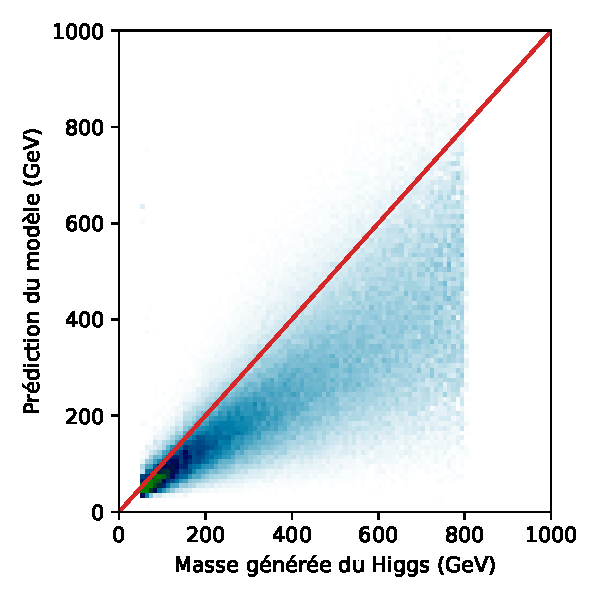
\includegraphics[width=.45\textwidth]{\PhDthesisdir/plots_and_images/my_plots/ML/from_ML_plots/DNNs_for_discussion/Mass_range/predicted_vs_answers_histo-NN-activation-softplus-batch_size-2048-mape-Adam-gu-inclusive-3-layers-1000-neurons.pdf}\vspace{-.5\baselineskip}}
\hfill
\subcaptionbox{Réponse.\label{subfig-reponse_Bsmr}}[.45\textwidth]
{\includegraphics[width=.45\textwidth]{\PhDthesisdir/plots_and_images/my_plots/ML/from_ML_plots/DNNs_for_discussion/Mass_range/model_response-NN-activation-softplus-batch_size-2048-mape-Adam-gu-inclusive-3-layers-1000-neurons.pdf}\vspace{-.5\baselineskip}}

\caption{Performances du modèle \Bsmr.}
\label{fig-Bsmr}
\end{figure}
\par
L'histogramme à deux dimensions des prédictions de \Bsmr\ en fonction de la vraie valeur de $m_{\higgsML}$,
figure~\ref{subfig-pred_vs_answ_Bsmr},
montre que les prédictions du modèle sont contenues dans l'intervalle d'entraînement,
à quelques exceptions près.
Dans l'intervalle d'entraînement, les prédictions sont cohérentes avec $m_{\higgsML}$,
la population de l'histogramme est proche de la première bissectrice ($\ypred=\ytrue$) en rouge.
%En dehors de cet intervalle, le comportement du modèle est proche d'une classification.
Les événements
avec $m_{\higgsML}<\SI{200}{\GeV}$ sont prédits vers \SI{230}{\GeV}
et ceux 
avec $m_{\higgsML}>\SI{500}{\GeV}$ sont prédits vers \SI{480}{\GeV}.
Un modèle ne peut donc pas être utilisé afin de prédire des masses en dehors de son intervalle d'entraînement.
\par
Afin d'obtenir un modèle pertinent dans l'optique d'une utilisation dans les analyses de CMS,
il est donc important d'utiliser un intervalle
contenant la gamme de masse des particules du modèle standard,
en particulier des bosons \Zboson\ et \higgs\ à \num{91.2} et \SI{125.1}{\GeV} respectivement.
Pour une recherche de bosons de Higgs supplémentaires de haute masse,
la limite supérieure de l'intervalle d'entraînement doit être la plus haute possible.
\subsubsection{Effet de bord}
\paragraph{Origine de l'effet de bord}
L'intervalle de masse utilisé pour l'entraînement du modèle B
s'étend de \num{50} à \SI{800}{\GeV}.
Comme discuté dans la section~\ref{chapter-ML-section-evt_gen},
il ne nous est pas possible de l'étendre avec la méthode utilisée pour générer les événements.
Or, il existe un effet de bord sur les prédictions du modèle B lié à cet intervalle.
La figure~\ref{subfig-pred_vs_answ_B-boundaries_effect} montre l'histogramme à deux dimensions des prédictions de B en fonction de la vraie valeur de $m_{\higgsML}$.
Pour $m_{\higgsML}>\SI{600}{\GeV}$, les prédictions de B saturent progressivement en dessous de \SI{800}{\GeV}.
De même, la réponse moyenne de B à basse masse, figure~\ref{subfig-reponse_model_B-boundaries_effect},
est de $\num{1.01}\pm\num{0.01}$ pour $\SI{80}{\GeV}<m_{\higgsML}<\SI{200}{\GeV}$.
En dessous de \SI{80}{\GeV}, la réponse moyenne augmente
et
la limite de l'écart-type inférieur (limite basse de la bande verte $\pm1\sigma$) passe de \num{0.8} à \num{1.0}.
\begin{figure}[h]
\centering

\subcaptionbox{Prédictions en fonction des valeurs vraies.\label{subfig-pred_vs_answ_B-boundaries_effect}}[.45\textwidth]
{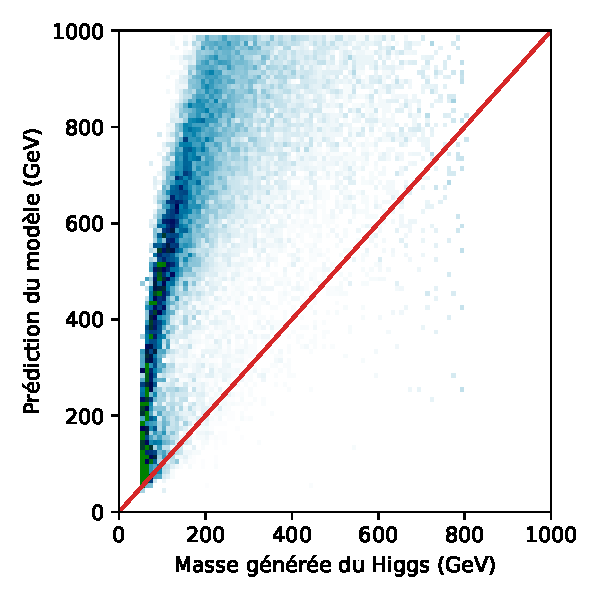
\includegraphics[width=.45\textwidth]{\PhDthesisdir/plots_and_images/my_plots/ML/from_ML_plots/trained_NNs_FastSim/DeepTau-inclusive/PuppiMET_with_METcov_j1j2jr_Nnu_Npu/predicted_vs_answers_histo-NN-ADAM_glorot_uniform-activation-softplus-batch_size-2048-mape-Adadelta-u-inclusive-3-layers-1000-neurons.pdf}\vspace{-.5\baselineskip}}
\hfill
\subcaptionbox{Réponse du modèle B à basse masse.\label{subfig-reponse_model_B-boundaries_effect}}[.45\textwidth]
{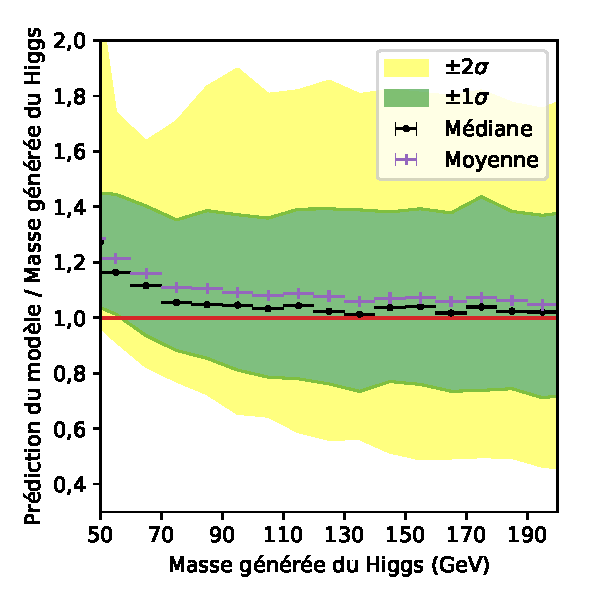
\includegraphics[width=.45\textwidth]{\PhDthesisdir/plots_and_images/my_plots/ML/from_ML_plots/trained_NNs_FastSim/DeepTau-inclusive/PuppiMET_with_METcov_j1j2jr_Nnu_Npu/model_response_lowmass-NN-ADAM_glorot_uniform-activation-softplus-batch_size-2048-mape-Adadelta-u-inclusive-3-layers-1000-neurons.pdf}\vspace{-.5\baselineskip}}

\caption{Performances du modèle B.}
\label{fig-B-boundaries_effect}
\end{figure}
\par
Ainsi, $m_{\higgsML}$ est surestimée à basse masse
et
sous-estimée à haute masse.
Il s'agit de l'effet de bord de l'intervalle de masse.
L'interprétation de cet effet est la suivante.
Chaque ensemble d'événements prédits à une valeur de \ypred\ donnée est une même famille du point de vue du DNN.
En termes de classification en un nombre infini de catégories au lieu de régression, cela revient à dire qu'une famille est donc une catégorie identifiée.
Sur la figure~\ref{fig-B-boundaries_effect-true_at_pred}
sont représentées les distributions de $\ytrue=m_{\higgsML}$
pour des valeurs de la masse prédite par le modèle $\ypred$ de
\num{400} (figure~\ref{subfig-true_at_pred_400}) et \SI{750}{\GeV} (figure~\ref{subfig-true_at_pred_750})
à $\pm\SI{5}{\GeV}$.
Il s'agit donc de tranches horizontales de l'histogramme de la figure~\ref{subfig-pred_vs_answ_B-boundaries_effect},
ce qui correspond à une famille d'événements selon le DNN.
\begin{figure}[h]
\centering

\subcaptionbox{Distribution de \ytrue\ pour $\ypred=\num{400}\pm\SI{5}{\GeV}$.\label{subfig-true_at_pred_400}}[.45\textwidth]
{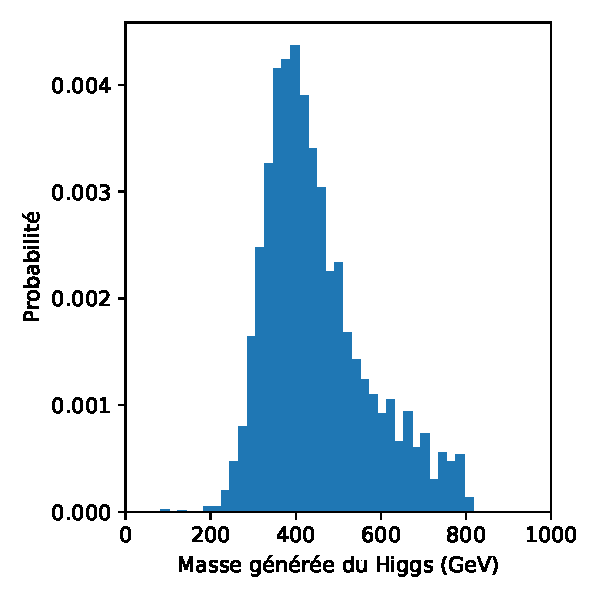
\includegraphics[width=.45\textwidth]{\PhDthesisdir/plots_and_images/my_plots/ML/from_ML_plots/DNNs_for_discussion/Mass_range/distributions/distribution-inclusive-Higgs_mass_gen-at_pred_mass_400weighted-is_test.pdf}\vspace{-.5\baselineskip}}
\hfill
\subcaptionbox{Distribution de \ytrue\ pour $\ypred=\num{750}\pm\SI{5}{\GeV}$.\label{subfig-true_at_pred_750}}[.45\textwidth]
{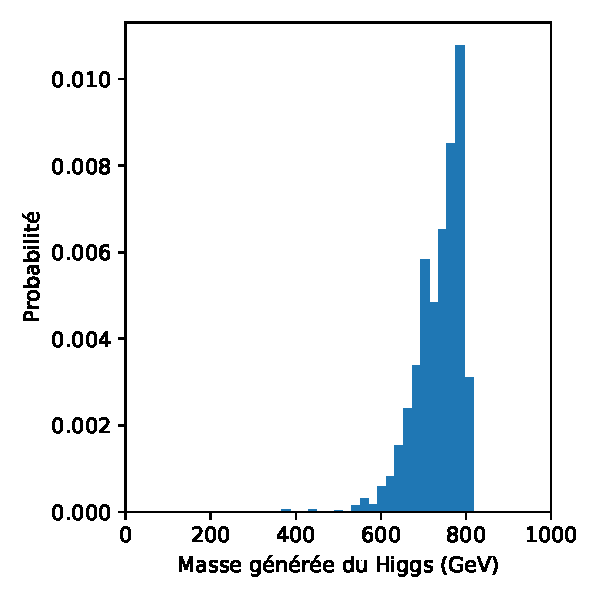
\includegraphics[width=.45\textwidth]{\PhDthesisdir/plots_and_images/my_plots/ML/from_ML_plots/DNNs_for_discussion/Mass_range/distributions/distribution-inclusive-Higgs_mass_gen-at_pred_mass_750weighted-is_test.pdf}\vspace{-.5\baselineskip}}

\caption{Distributions de \ytrue\ à \ypred\ fixée.}
\label{fig-B-boundaries_effect-true_at_pred}
\end{figure}
\par
Loin des bords de l'intervalle d'entraînement,
figure~\ref{subfig-true_at_pred_400},
la distribution de \ytrue\ pour une famille est complète.
Des deux côtés de la valeur centrale, les queues de la distribution sont présentes.
Lors de l'entraînement,
le DNN \og apprend \fg{} à prédire pour les événements de cette famille
la valeur de \ypred\ minimisant la fonction de coût sur cette distribution.
Nous obtenons dans ce cas une valeur proche de \SI{400}{\GeV}, ce qui est correct.
%Il est à noter que certains événements générés à $m_{\higgsML}=\SI{800}{\GeV}$ font partie de cette famille, ce qui est lié à la résolution du modèle.
\par
Au niveau du bord à haute masse,
figure~\ref{subfig-true_at_pred_750},
l'absence d'événements au-delà de \SI{800}{\GeV} donne une distribution tronquée de \ytrue\ pour une famille donnée.
Seule l'extrémité à basse masse de la queue de la distribution est présente.
Par conséquent,
le DNN ne connaît que les basses masses de cette famille,
il est ainsi tout à fait cohérent qu'il en sous-estime la masse.
La minimisation de la fonction de coût mène donc à des prédictions biaisées.
Si les événements au-delà de \SI{800}{\GeV} étaient présents dans cette famille,
la distribution serait plus étendue vers les hautes masses,
et la minimisation de la fonction de coût mènerait donc le DNN à prédire une masse plus élevée.
L'effet est inversé pour le bord à basse masse, d'où la surestimation.
\paragraph{Principe de la correction}
La minimisation de la fonction de coût est donc réalisée correctement, mais sur des familles d'événements tronquées.
Afin de contrer cet effet,
l'idée retenue est de reformer des familles équilibrées
en les tronquant de manière symétrique par rapport à la valeur de \ytrue\ devant leur correspondre.
La figure~\ref{subfig-mirrored_cut-2D_histo} illustre le principe de cette coupure symétrique.
\begin{figure}[h]
\centering

\subcaptionbox{Principe de la coupure symétrique à haute masse.\label{subfig-mirrored_cut-2D_histo}}[.45\textwidth]
{\includegraphics[width=.45\textwidth]{\PhDthesisdir/plots_and_images/my_plots/ML/custom_loss-illustrations/distance_and_mirror.tex}\vspace{-.5\baselineskip}}
\hfill
\subcaptionbox{Distribution de \ytrue\ pour $\ypred=\num{750}\pm\SI{5}{\GeV}$ avec coupure symétrique.\label{subfig-mirrored_cut-true_at_pred_750}}[.45\textwidth]
{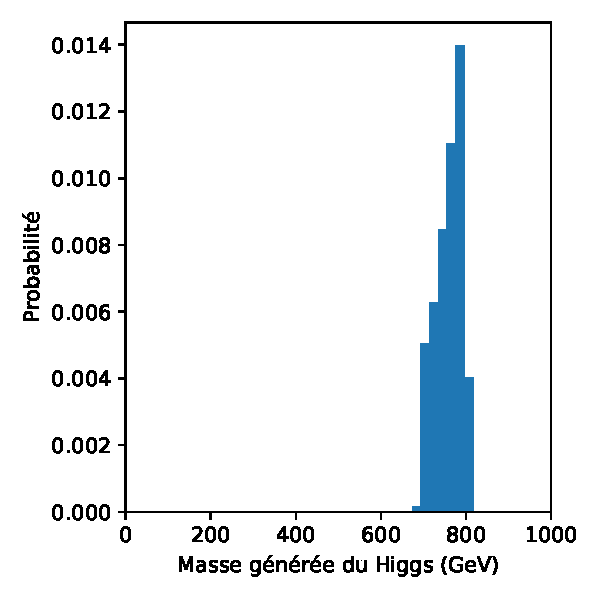
\includegraphics[width=.45\textwidth]{\PhDthesisdir/plots_and_images/my_plots/ML/from_ML_plots/DNNs_for_discussion/Mass_range/distributions/distribution-inclusive-Higgs_mass_gen-mirrored_cut_at_pred_mass_750weighted-is_test.pdf}\vspace{-.5\baselineskip}}

\caption{Mise en place de la coupure symétrique.}
\label{fig-B-boundaries_effect-mirrored_cut}
\end{figure}
\par
La troncature des familles due à l'extrémité de l'intervalle à \SI{800}{\GeV}
est symétrisée par rapport au centre de valeur \ytrue\ devant correspondre à chaque famille.
Ainsi, tout événement d'une famille (tranche horizontale)
situé à une distance $d$ de la valeur centrale à prédire (sur la diagonale rouge)
plus grande que la distance de cette valeur centrale à
l'extrémité de l'intervalle (trait orange vertical)
est rejeté de l'entraînement.
La distribution de la famille de la figure~\ref{subfig-true_at_pred_750}
symétrisée par troncature selon cette méthode est présentée sur la figure~\ref{subfig-mirrored_cut-true_at_pred_750}.
La valeur de la fonction de coût sur cette distribution n'est plus minimale pour la valeur prédite par le modèle,
elle l'est en revanche pour une valeur prédite plus élevée.
Le modèle actuel sous-estimant $m_{\higgsML}$ à haute masse,
cette correction doit donc permettre d'obtenir un nouveau modèle avec une réponse plus proche de 1.
\paragraph{Modification de la fonction de coût}
Une coupure symétrique est également mise en place pour les basses masses.
Cinq zones peuvent être définies dans le plan $(\ytrue, \ypred)$:
\begin{description}
\item[Zone 1] $\ytrue < \SI{50}{\GeV}$:\\
absence d'événements due à la masse minimale de l'entraînement;
\item[Zone 2] $\ytrue > \SI{800}{\GeV}$:\\
absence d'événements due à la masse maximale de l'entraînement;
\item[Zone 3] $\abs{\ypred - \ytrue} > \abs{\SI{800}{\GeV} - \ypred}$:\\
zone d'exclusion à haute masse;
\item[Zone 4] $\abs{\ypred - \ytrue} > \abs{\SI{50}{\GeV} - \ypred}$:\\
zone d'exclusion à basse masse;
\item[Zone 5] zone centrale.
\end{description}
\begin{wrapfigure}{R}{.45\textwidth}
\centering
\includegraphics[width=.45\textwidth]{\PhDthesisdir/plots_and_images/my_plots/ML/custom_loss-illustrations/areas.tex}
\caption{Zones considérées pour l'entraînement.}
\label{fig-B-boundaries_effect-mirrored_cut-areas}
\end{wrapfigure}
\par\noindent
Ces zones sont illustrées en figure~\ref{fig-B-boundaries_effect-mirrored_cut-areas}.
Dans la zone centrale, la fonction de coût est utilisée de manière classique, sans changement.
Dans les zones 3 et 4 d'exclusion en revanche,
afin de ne pas prendre en compte les événements comme prévu afin de symétriser les bords de l'intervalle d'entraînement au sein d'une famille,
la fonction de coût est rendue égale à zéro.
En d'autres termes, nous procédons au changement
$\Loss=\LossMAPE\to\Loss'$ avec
\begin{equation}
\Loss' = \LossMAPE \times
\left\lbrace
\begin{aligned}
0 \quad & \text{si $(\ytrue, \ypred)\in$ zones 3 ou 4}\\
1 \quad & \text{sinon}
\end{aligned}
\right.
\mend
\end{equation}
La fonction de coût ainsi obtenue ne respecte pas la condition
\begin{equation}
\Loss(\ytrue, \ypred) = 0 \Leftrightarrow \ytrue = \ypred
\mend[,]
\end{equation}
des problèmes de convergence lors de l'entraînement peuvent survenir.
C'est effectivement ce que nous avons pu observer lors de la mise en place de cette fonction de coût
avec la condition d'exclusion de la zone 4.
Nous avons alors choisi de multiplier la valeur de la fonction de coût par \num{0.1} dans la zone 4 au lieu de 0.
De plus, nous avons observé que la multiplication de $\LossMAPE$ par la racine de \ytrue,
conjointement avec les conditions d'exclusion,
permettait d'améliorer encore la réponse du modèle.
La fonction de coût ainsi utilisée est
\LossMAPEsqrtb, définie par
\begin{equation}
\LossMAPEsqrtb(\ytrue, \ypred)
=
\LossMAPEsqrt(\ytrue, \ypred)
\times
\left\lbrace
\begin{aligned}
0 \quad & \text{si $(\ytrue, \ypred)\in$ zone 3}\\
\num{0.1} \quad & \text{si $(\ytrue, \ypred)\in$ zone 4}\\
1 \quad & \text{sinon}
\end{aligned}
\right.
\label{eq-LossMAPEsqrtb}
\end{equation}
avec
\begin{align}
\LossMAPEsqrt(\ytrue, \ypred)
&=
\LossMAPE(\ytrue, \ypred) \times \sqrt{\ytrue}
=
\abs{\frac{\ypred-\ytrue}{\ytrue}} \times \sqrt{\ytrue}
\nonumber\\\Leftrightarrow
\LossMAPEsqrt(\ytrue, \ypred)
&=
\abs{\frac{\ypred-\ytrue}{\sqrt{\ytrue}}}
\mend
\end{align}
\paragraph{Nouveau modèle obtenu}
Le nouveau modèle obtenu, noté B', est comparé à B
sur la figure~\ref{fig-B_Bprime_Bpprime-boundaries_effect}.
\begin{figure}[p]
\centering

\subcaptionbox{Réponse du modèle B.\label{subfig-B-B_Bprime_Bpprime}}[.45\textwidth]
{\includegraphics[width=.45\textwidth]{\PhDthesisdir/plots_and_images/my_plots/ML/from_ML_plots/trained_NNs_FastSim/DeepTau-inclusive/PuppiMET_with_METcov_j1j2jr_Nnu_Npu/model_response-NN-ADAM_glorot_uniform-activation-softplus-batch_size-2048-mape-Adadelta-u-inclusive-3-layers-1000-neurons.pdf}\vspace{-.5\baselineskip}}
\hfill
\subcaptionbox{Réponse du modèle B à basse masse.\label{subfig-B_lowmass-B_Bprime_Bpprime}}[.45\textwidth]
{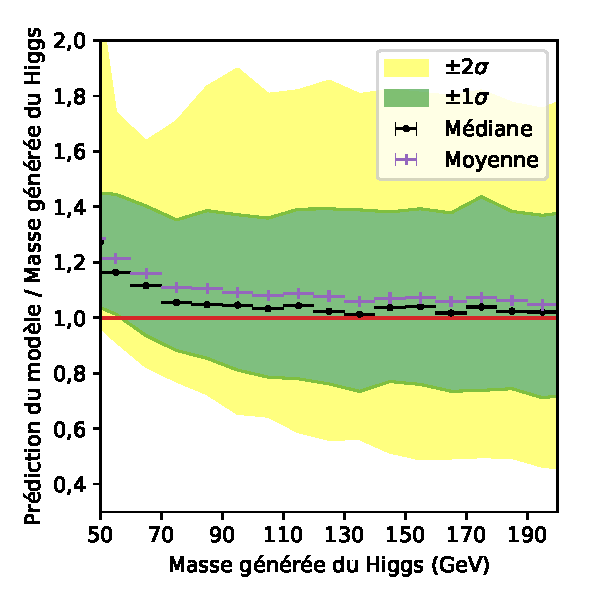
\includegraphics[width=.45\textwidth]{\PhDthesisdir/plots_and_images/my_plots/ML/from_ML_plots/trained_NNs_FastSim/DeepTau-inclusive/PuppiMET_with_METcov_j1j2jr_Nnu_Npu/model_response_lowmass-NN-ADAM_glorot_uniform-activation-softplus-batch_size-2048-mape-Adadelta-u-inclusive-3-layers-1000-neurons.pdf}\vspace{-.5\baselineskip}}

\subcaptionbox{Réponse du modèle B'.\label{subfig-Bprime-B_Bprime_Bpprime}}[.45\textwidth]
{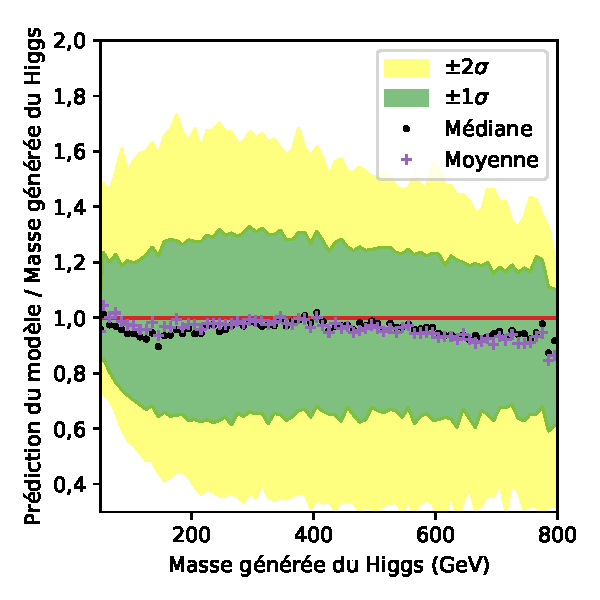
\includegraphics[width=.45\textwidth]{\PhDthesisdir/plots_and_images/my_plots/ML/from_ML_plots/trained_NNs_FastSim/DeepTau-inclusive/PuppiMET_with_METcov_j1j2jr_Nnu_Npu/model_response-NN-activation-softplus-batch_size-2048-mapesqrt_b-Adam-gu-inclusive-3-layers-1000-neurons.pdf}\vspace{-.5\baselineskip}}
\hfill
\subcaptionbox{Réponse du modèle B' à basse masse.\label{subfig-Bprime_lowmass-B_Bprime_Bpprime}}[.45\textwidth]
{\includegraphics[width=.45\textwidth]{\PhDthesisdir/plots_and_images/my_plots/ML/from_ML_plots/trained_NNs_FastSim/DeepTau-inclusive/PuppiMET_with_METcov_j1j2jr_Nnu_Npu/model_response_lowmass-NN-activation-softplus-batch_size-2048-mapesqrt_b-Adam-gu-inclusive-3-layers-1000-neurons.pdf}\vspace{-.5\baselineskip}}

\subcaptionbox{Réponse du modèle B".\label{subfig-Bpprime-B_Bprime_Bpprime}}[.45\textwidth]
{\includegraphics[width=.45\textwidth]{\PhDthesisdir/plots_and_images/my_plots/ML/from_ML_plots/selected_NNs_FastSim/DeepTau-inclusive-1TeV/PuppiMET_with_METcov_j1j2jr_Nnu_Npu/plots_up_to_800/model_response-NN-activation-softplus-batch_size-2048-mapesqrt_b-Adam-gu-inclusive-3-layers-1000-neurons.pdf}\vspace{-.5\baselineskip}}
\hfill
\subcaptionbox{Réponse du modèle B" à basse masse.\label{subfig-Bpprime_lowmass-B_Bprime_Bpprime}}[.45\textwidth]
{\includegraphics[width=.45\textwidth]{\PhDthesisdir/plots_and_images/my_plots/ML/from_ML_plots/selected_NNs_FastSim/DeepTau-inclusive-1TeV/PuppiMET_with_METcov_j1j2jr_Nnu_Npu/plots_up_to_800/model_response_lowmass-NN-activation-softplus-batch_size-2048-mapesqrt_b-Adam-gu-inclusive-3-layers-1000-neurons.pdf}\vspace{-.5\baselineskip}}

\caption{Comparaison des modèles B, B' et B".}
\label{fig-B_Bprime_Bpprime-boundaries_effect}
\end{figure}
Pour des masses inférieures à \SI{70}{\GeV},
la réponse médiane de B', en figure~\ref{subfig-Bprime_lowmass-B_Bprime_Bpprime},
est égale à 1 alors que celle de B, en figure~\ref{subfig-B_lowmass-B_Bprime_Bpprime},
est sujette à l'effet de bord.
À haute masse,
la réponse de B' en figure~\ref{subfig-Bprime-B_Bprime_Bpprime} est également plus proche de 1
que celle de B, en figure~\ref{subfig-B-B_Bprime_Bpprime}.
L'utilisation de  \LossMAPEsqrt\ comme fonction de coût permet donc de
supprimer l'effet de bord à basse masse
et de le réduire à haute masse.
\paragraph{Exploitation de la queue à haute masse des événements générés}
Lors de la génération des événements à haute masse, la largeur du boson de Higgs permet d'obtenir des événements avec $m_{\higgsML}$ supérieure à \SI{800}{\GeV}, comme discuté en section~\ref{chapter-ML-section-evt_gen}.
Jusqu'ici, nous ne considérerions que les événements tels que
$\SI{50}{\GeV}\leq m_{\higgsML}\leq \SI{800}{\GeV}$.
L'inclusion de la queue à haute masse des événements générés permet d'étendre artificiellement l'intervalle d'entraînement jusqu'à \SI{1}{\TeV}.
Le biais éventuel dû à la faible quantité d'événements au-delà de \SI{800}{\GeV} est évité grâce à la pondération présentée dans la section~\ref{chapter-ML-section-evt_gen}.
De même, les définitions des cinq zones utilisées pour déterminer la fonction de coût sont adaptées à la nouvelle valeur maximale de $m_{\higgsML}$ fixée à \SI{1}{\TeV}.
Le modèle B" ainsi obtenu est est comparé à B'
sur la figure~\ref{fig-B_Bprime_Bpprime-boundaries_effect}.
La réponse à basse masse de B", figure~\ref{subfig-Bpprime_lowmass-B_Bprime_Bpprime},
est semblable à celle de B', figure~\ref{subfig-Bprime_lowmass-B_Bprime_Bpprime},
ce qui est attendu.
En revanche, la réponse moyenne de B" à haute masse, figure~\ref{subfig-Bpprime-B_Bprime_Bpprime},
est de $\num{1.00}\pm\num{0.04}$
contre $\num{0.93}\pm\num{0.07}$ pour B', figure~\ref{subfig-Bprime-B_Bprime_Bpprime}.
Enfin, la résolution relative de B' est de \SI{22}{\%}, celle de B" de \SI{25}{\%}.
%\medskip\par
L'utilisation de la fonction de coût modifiée \LossMAPEsqrtb\
et des événements entre \SI{800}{\GeV} et \SI{1}{\TeV} obtenus grâce à la largeur de \higgsML\
permet ainsi de ramener la réponse moyenne du modèle à des valeurs de $\num{1.00}\pm\num{0.05}$
pour des valeurs de $m_{\higgsML}$ allant de \num{80} à \SI{800}{\GeV}.
\subsection{Modèle final}
Le modèle B" que nous avons construit
est donc entraîné sur des événements $\higgsML\to\tau\tau$
où \higgsML\ est le boson de Higgs du modèle standard \higgs\ avec une masse modifiée
entre \num{50} et \SI{800}{\GeV},
avec addition d'empilement selon le profil de l'année 2017,
dont la sélection est réalisée selon la procédure décrite section~\ref{chapter-ML-section-evt_gen}.
En particulier, l'algorithme \DEEPTAU~\cite{CMS-DP-2019-033} est utilisé pour l'identification des taus hadroniques.
La largeur de \higgsML\ permet d'exploiter des événements où sa masse effective est supérieure à \SI{800}{\GeV}, jusqu'à \SI{1}{\TeV}.
La gamme d'utilisation de notre modèle est toutefois considérée comme allant de \num{50} à \SI{800}{\GeV} uniquement.
Les hyper-paramètres de B" sont ceux de B à l'exception de la fonction de coût:
\begin{itemize}
\item 3 couches cachées;
\item \num{1000} neurones par couche cachée;
\item fonction d'activation Softplus, $x\mapsto\ln(1+\eexp{x})$;
\item algorithme d'optimisation Adam, présenté en section~\ref{chapter-ML-section-DNN-training-optimizers};
\item fonction de coût \LossMAPEsqrtb, définie équation~\eqref{eq-LossMAPEsqrtb};
\item initialisation des poids selon le mode \og Glorot Uniforme \fg~\cite{glorot};
\item 27 variables d'entrée données en section~\ref{chapter-ML-section-evt_gen-inputs}.
\end{itemize}
\par
L'utilisation de B" dans les analyses de CMS est abordé dans la section suivante.